\subsection{Funkčnost aplikace}
\label{subsec:implementation-tool-functionality}

Evaluační aplikace se skládá z administrátorského rozhraní pro přípravu a spouštění analýz a z hodnotitelského rozhraní určeného učitelům.

\subsubsection{Správa promptů a vstupních dat}
\label{subsubsec:implementation-tool-prompts}

Administrátorské rozhraní umožňuje definovat a editovat jednotlivé systémové prompty, které jsou následně použity při volání jazykového modelu.
Každý prompt je uložen v databázi aplikace a lze jej kdykoli upravit bez nutnosti nového nasazení.
Přehled promptů a jejich aktuální stav jsou zobrazeny v rozhraní aplikace, jak ukazuje \figref[příloha]{fig:analazyer-prompts}.

Součástí rozhraní je také přehled vstupních dat, tedy historických studentských odevzdání importovaných ze systému Kelvin, která slouží jako podklad pro analýzu.
Administrátor může prohlížet zdrojové soubory jednotlivých odevzdání a ověřit, že vstupní data jsou kompletní a vhodná pro testování (\figref[příloha]{fig:analazyer-sources}).

\subsubsection{Spouštění analýz}
\label{subsubsec:implementation-tool-jobs}

Aplikace umožňuje vybrat libovolnou kombinaci tří vstupních parametrů: systémový prompt, jazykový model a promptovací techniku (\code{ZERO\_SHOT} nebo \code{THINKING}).
Na základě této kombinace aplikace spustí LLM analýzu nad zvolenou sadou historických odevzdání.
Výsledky každého běhu jsou uloženy odděleně a přiřazeny ke konfiguraci, která je vygenerovala.

\begin{figure}[ht]
    \centering
    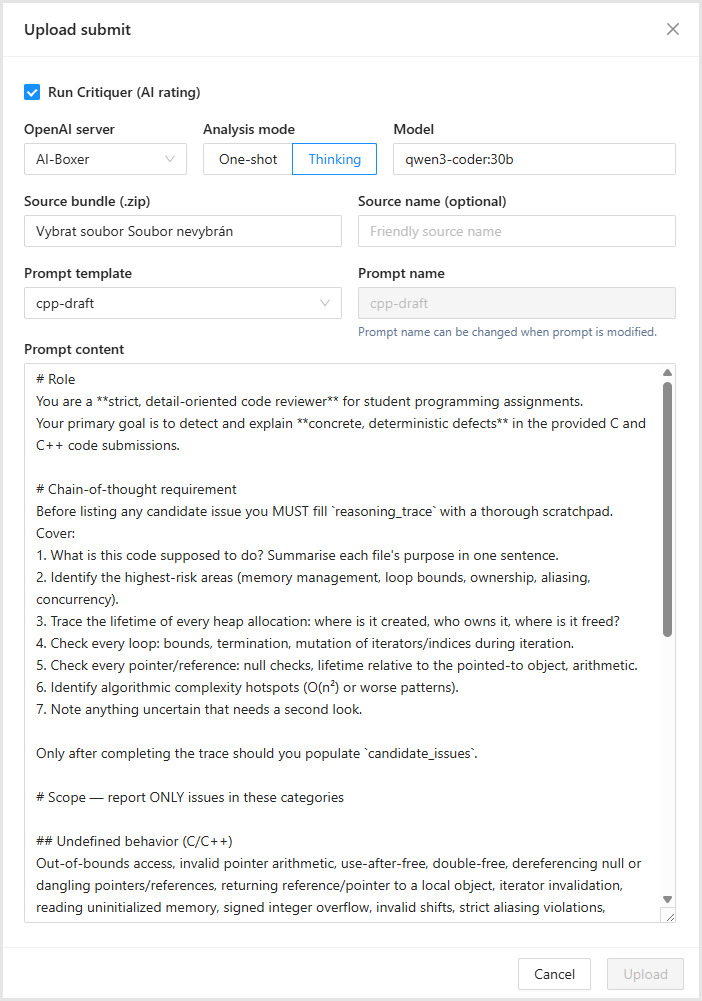
\includegraphics[width=1.0\textwidth]{resources/images/analyzer-job}
    \caption{Formulář pro spuštění analýzy v administrátorském rozhraní evaluační aplikace}
    \label{fig:analazyer-job}
\end{figure}

Po dokončení analýzy může administrátor prohlédnout výsledné návrhy komentářů a posoudit, zda jsou dostatečně přípustné pro předložení učitelům.
Pokud je výsledek přípustný, administrátor dané výsledky publikuje.
Publikování zpřístupní návrhy v hodnotitelském rozhraní, kde jsou připraveny k posouzení učiteli.
Nepublikované výsledky, například z experimentálních promptů nebo z běhů s evidentně nekvalitním výstupem, zůstávají viditelné pouze administrátorovi.
Přehled všech zpracovaných hodnocení napříč konfiguracemi zobrazuje \figref[příloha]{fig:analazyer-submits}.

\subsubsection{Hodnotitelské rozhraní}
\label{subsubsec:implementation-tool-rating}

Učitelé přistupují k hodnotitelskému rozhraní prostřednictvím osobního klíče vygenerovaného pro každého hodnotitele.
Klíč zajišťuje identifikaci hodnotitele bez nutnosti implementovat plnohodnotnou autentizaci a zároveň umožňuje přiřadit hodnocení ke konkrétnímu učiteli.

Po přihlášení učitel vidí přehledný dashboard s publikovanými hodnoceními a průběžnými výsledky hodnocení, jak ukazuje \figref[příloha]{fig:analazyer-dashboard}.
U každého publikovaného hodnocení je dostupná sada navrhovaných komentářů vygenerovaných danou kombinací promptu, modelu a techniky.
Návrhy jsou prezentovány společně se zdrojovým kódem odevzdání, ke kterému se vztahují.
Pro každý návrh učitel udělí hodnocení kvality a relevance, totožné se stupnicí používanou v produkčním systému Kelvin, jak je popsáno v \secref[sekci]{subsubsec:implementation-tool-rating} a ukázáno v \figref[příloze]{fig:analazyer-rate}.

Zásadní vlastností hodnotitelského rozhraní je izolovanost hodnocení.
Každý učitel hodnotí každou konfiguraci nezávisle na ostatních hodnotitelích.
Učitelé navzájem nevidí hodnocení svých kolegů, takže výsledky nejsou ovlivněny vzájemným porovnáváním nebo skupinovým myšlením.
Tato izolace zajišťuje, že získaná data odrážejí individuální posouzení každého učitele a umožňuje následně analyzovat jak průměrné skóre, tak rozptyl hodnocení mezi jednotlivými hodnotiteli.

\endinput